\section{钳口三维建模}

\begin{figure}[htbp]
\centering
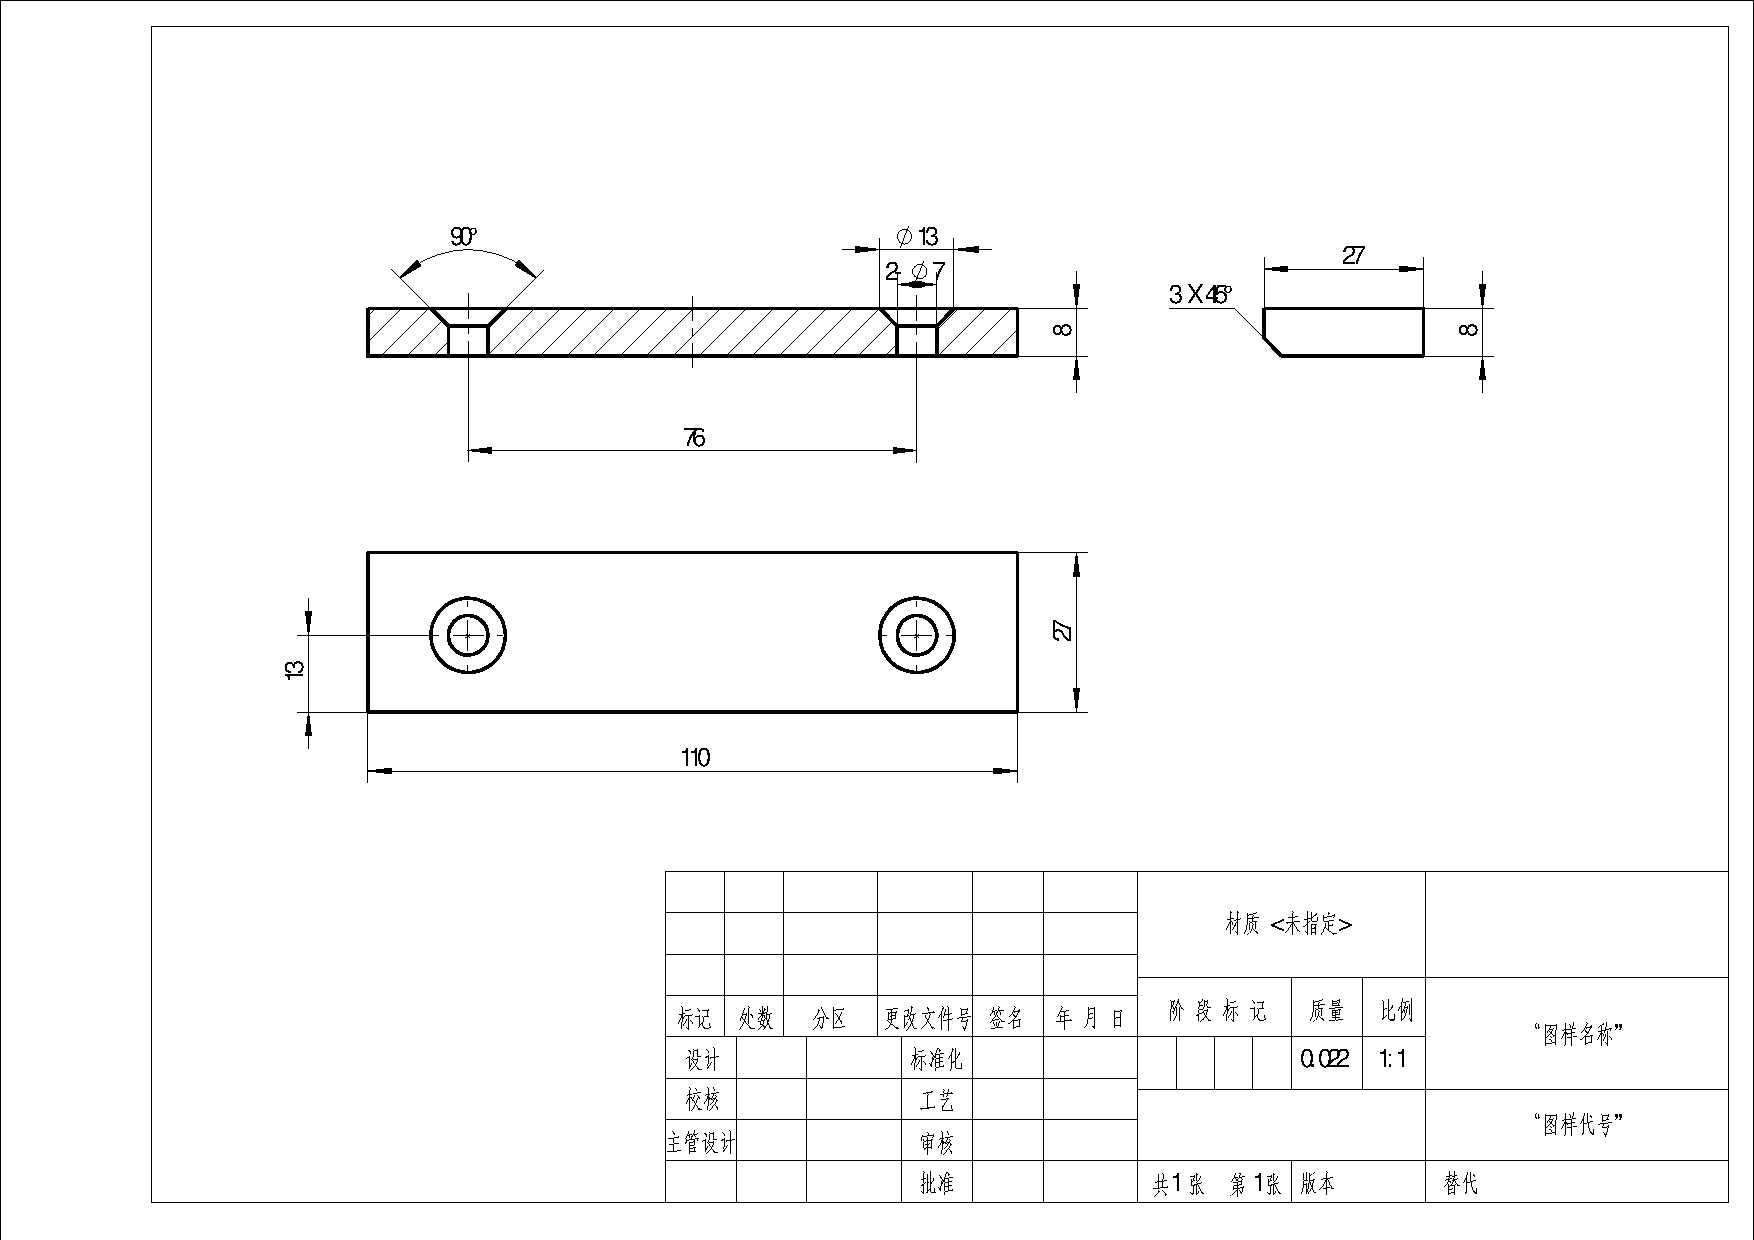
\includegraphics[width=0.8\textwidth]{taihuqianko.pdf}
\caption{套筒零件图}\label{fig:taihuqianko}
\end{figure}

在台虎钳的固定钳身和活动钳身上,均装有钢制钳口,并用螺钉固定。钳口的工作面上制有交叉的网纹,使工件夹紧后不易产生滑动。钳口经过热处理淬硬,具有较好的耐磨性。其具体的零件尺寸如图\ref{fig:taihuqianko}所示。
\endinput